\chapter{Understanding Metamaterial Mechanisms}
\label{chapter:Understanding-metamaterial-mechanisms}

% The recent rise of widely accessible fabrication machines, such as 3D printers or laser cutters, generated interest in non-experts to create and design their own devices. Their strive towards a future of personal- rather than mass-fabrication is supported by HCI researchers [4], who investigate techniques to directly interact with the machine [29][32][50], use real-world objects for content creation [48][49] or embed mechanisms [52] and electronics [38]. These works were mainly concerned with creating the outside shape of 3D objects.

% 3D printing technology, however, is unique in that it allows users to freely arrange matter in space. Researchers used this property to generate internal structures that, e.g., optimize the strength-to-weight ratio of 3D objects [25], allow arbitrarily shaped objects to spin [3], or to float in pre-defined poses [34].

% Pushing this idea further, researchers engineer microstructures that deform in a desired way. These structures are usually arranged on a regular grid and together define the properties of the material they form [5]. This concept is known as metamaterials. Such metamaterial structures can be designed to change the materials’ elasticity [40], to absorb energy [12][43], or to change their shape [28]. 

% Recently, Ion et al. [18] pushed the concept of metamaterials further by going beyond materials and create complete mechanisms from cellular structures. Their mechanisms consist of two types of cells that are carefully arranged to move in concert to achieve the macroscopic mechanical movement. With their novel concept, they showed example objects including a door latch or a Jansen walker. However, it remains unclear what types of mechanisms can be implemented with such metamaterials.

In the previous chapter, we pushed the concept of metamaterials further by going beyond materials and create complete mechanisms from cellular structures. 
% Their mechanisms consist of two types of cells that are carefully arranged to move in concert to achieve the macroscopic mechanical movement.
We demonstrated our novel concept with example objects including a door latch or a Jansen walker. However, it remained unclear what types of mechanisms can be implemented with such metamaterials.

In this work, we investigate the underlying working principles of such metamaterial mechanisms. To do so, we analyze the interaction of the two types of cells, identify the underlying topological constraints of metamaterial mechanisms, and ultimately implement this domain knowledge into a computational design tool for non-expert users.

\begin{figure} [h]
    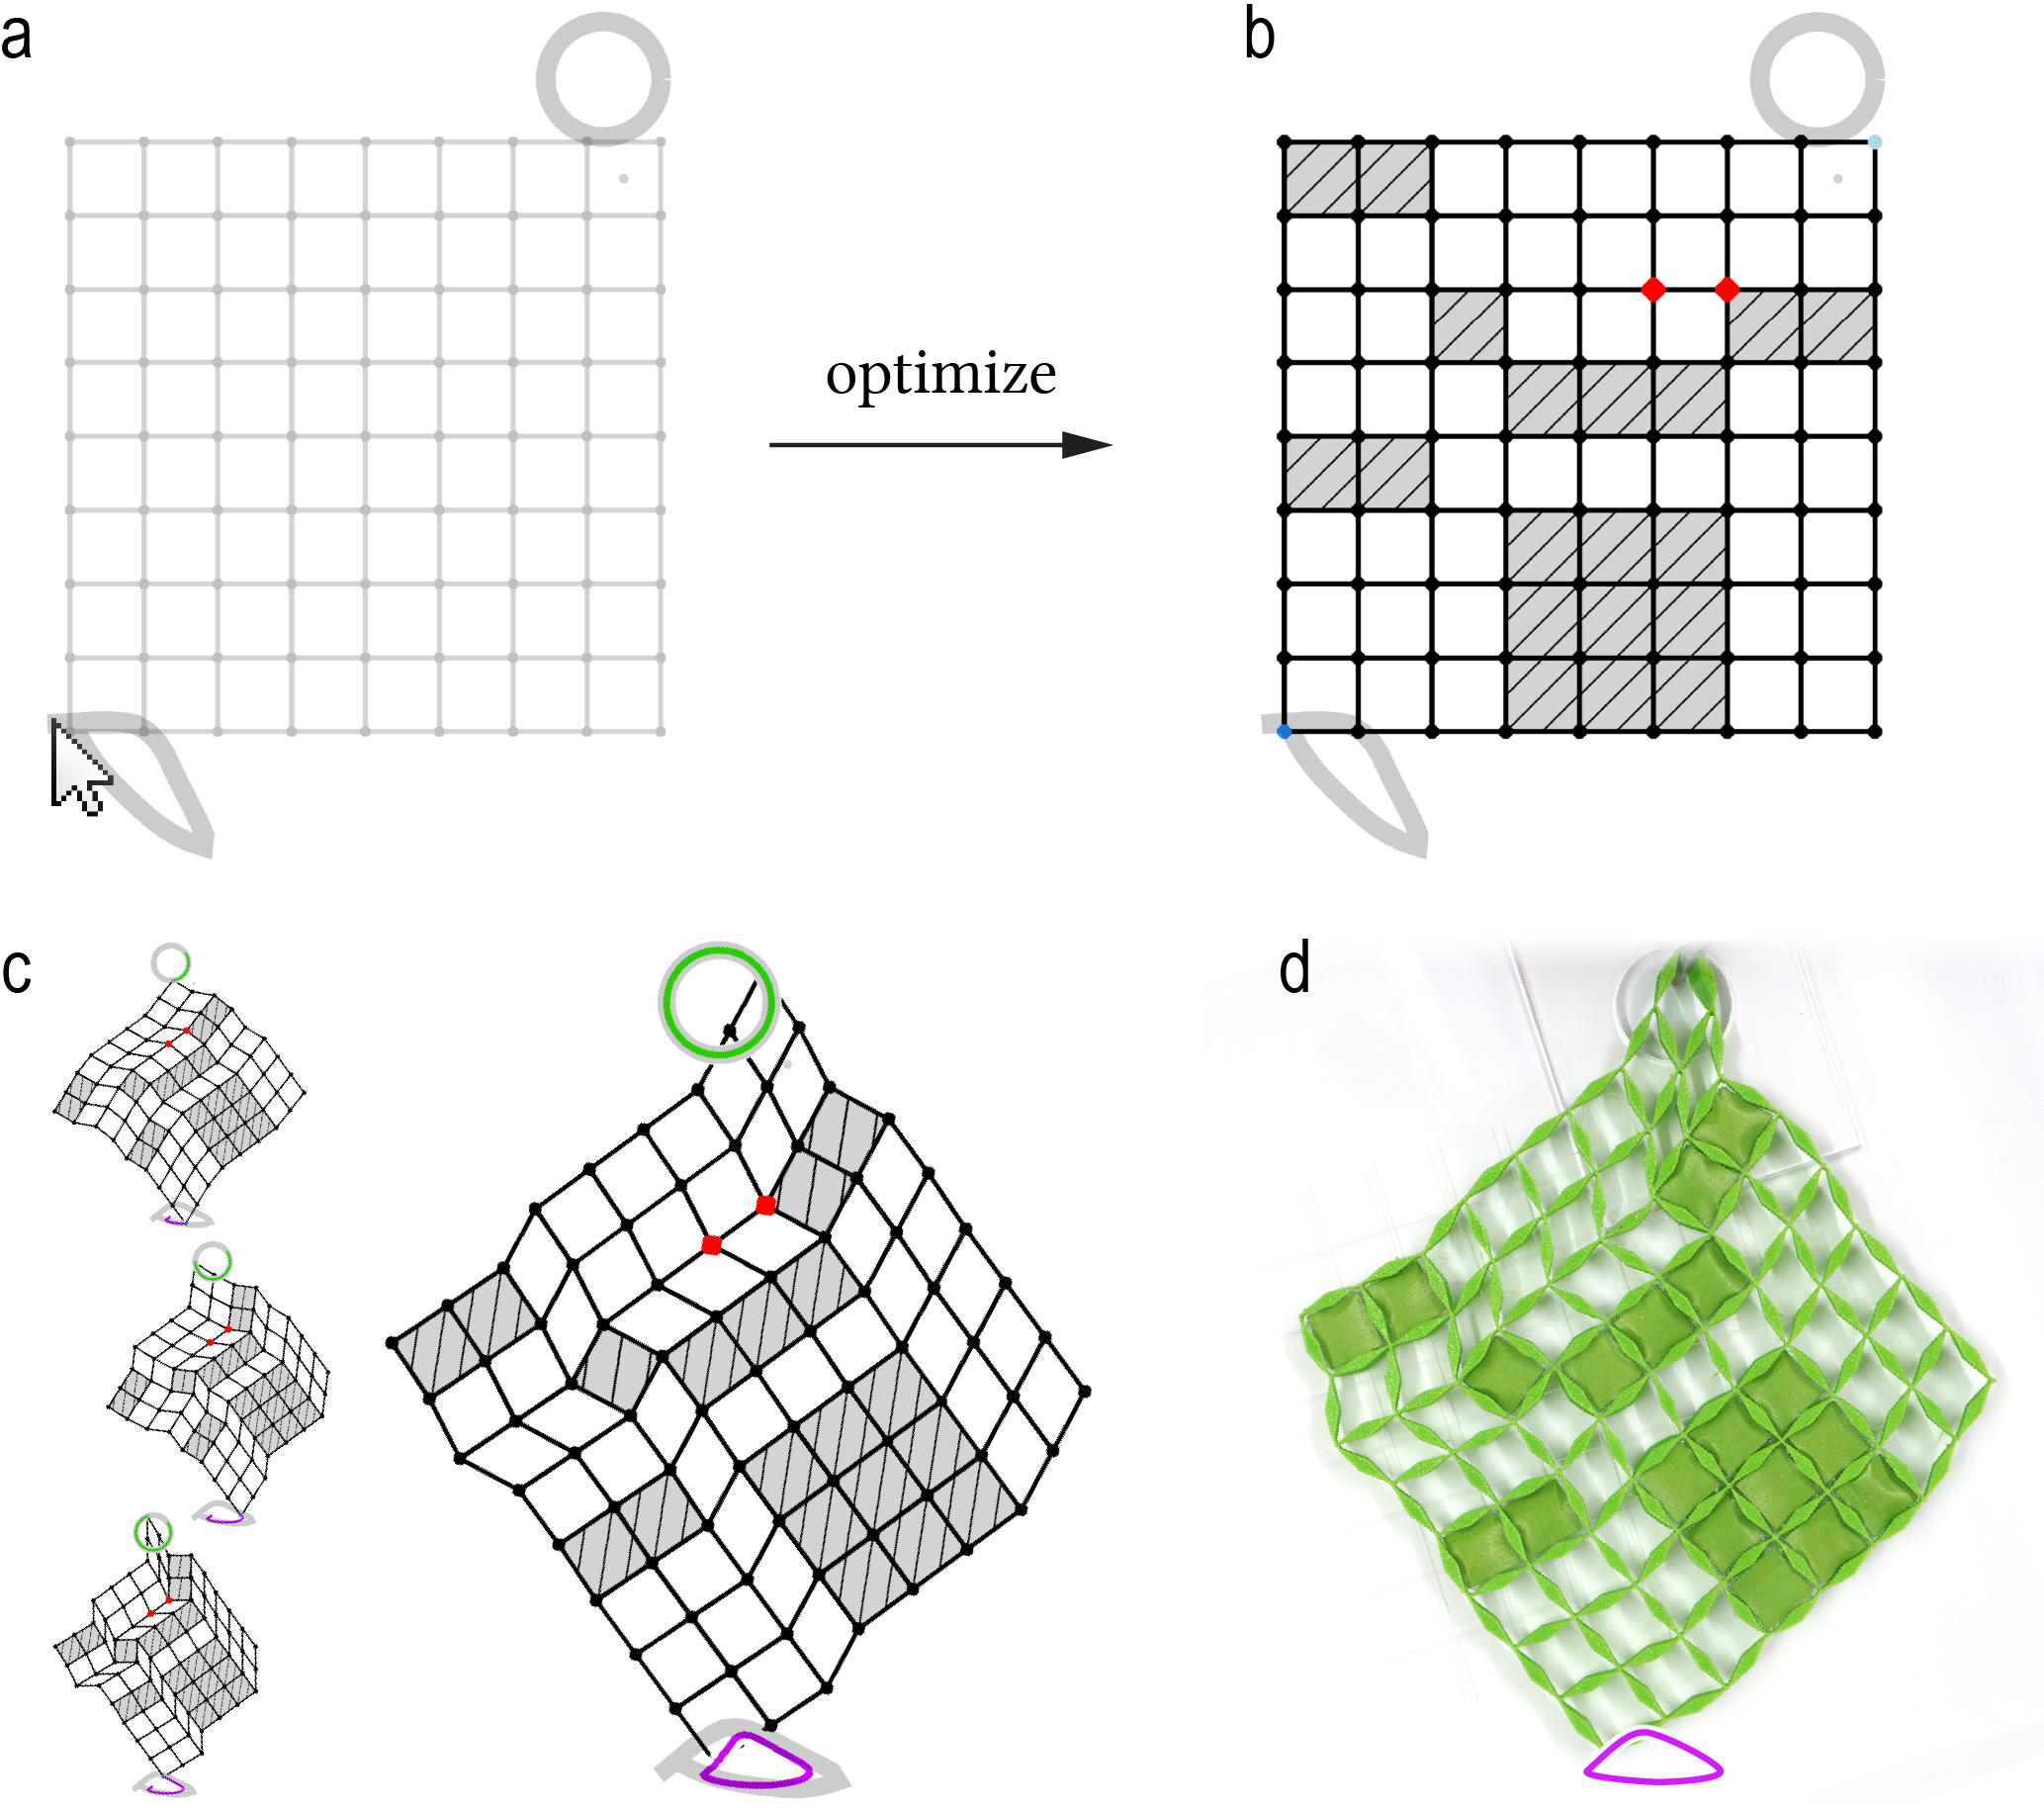
\includegraphics[width=\textwidth]{chapters/understanding-metamaterial-mechanisms-FIG/1-editor-and-walker.pdf}
    \caption[Short figure name.]{We define the underlying working principles of metamaterial mechanisms, which allows us to implement a computational design tool. (a) It takes user-drawn paths and (b) optimizes the cell configuration which implements the transformation. (c) In this example, we show the leg of a walker. (d) The fabricated result matches the optimized motion closely.
    \label{fig:1-editor-walker}}
\end{figure}


\section{Motivation \& challenges}

In this work, we set out to understand the underlying mechanisms that inform the design of metamaterial mechanisms. Such metamaterial mechanisms, as we introduced earlier in Chapter \ref{chapter:analog-metamaterials}, implement a transformation of an input movement to an output movement, such as in Figure \ref{fig:2-compare-doorlatch} with the retraction of the bolt when the door handle is pushed down.

\begin{figure} [h]
    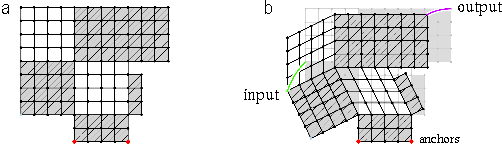
\includegraphics[width=\textwidth]{chapters/understanding-metamaterial-mechanisms-FIG/2-comparison-doorlatch.pdf}
    \caption[Short figure name.]{(a) Metamaterial mechanisms are implemented by their cell structure to create, e.g., this door latch, from a single block of material. (b) The microstructure implements a transformation from the green input path (pushing the handle) to the pink output path (retracting the bolt).
    \label{fig:2-compare-doorlatch}}
\end{figure}

Metamaterial mechanisms combine two types of cells on a regular grid. The individual cells (see Figure 3), are very simple---they are rigid or can shear. These cells are careful arranged within the material to play together in a well-defined way to implement the mechanism.

\begin{figure} [h]
    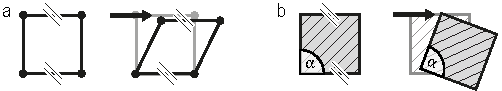
\includegraphics[width=\textwidth]{chapters/understanding-metamaterial-mechanisms-FIG/3-individual-cells.pdf}
    \caption[Short figure name.]{Metamaterial mechanisms consist of simple cells: shearing cells and rigid cells. (a) Shearing cells constrain their opposing edges to remain parallel and (b) rigid cells additionally maintain their angle.
    \label{fig:3-individual-cells}}
\end{figure}

In the remainder of this chapter, we will discuss metamaterial mechanisms on a higher level of abstraction, i.e., we will leave out the device applying the metamaterial and instead focus just on the cell structure and the transformation it implements.


\subsection{Understanding cell constraints and how they interact}

To achieve the movement that implements the desired mechanism, the cells need to be arranged on a grid to play together in a well-defined way. More formally, “play together” means that each individual cell has constraints that it propagates to its neighbors. For example, opposing edges of shear cells remain parallel (parallelism constraints) and rigid cells additionally maintain their angle (angle constraints). Since the cells are connected in two dimensions, their constraints can interact. We illustrate such constraint interactions in Figure \ref{fig:4-constraint-interaction}. This example shows how adding a single cell (marked in blue) prevents 7 other shear cells on the grid from shearing.

\begin{figure} [h]
    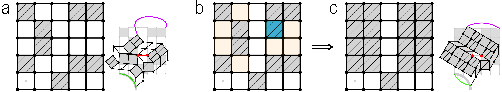
\includegraphics[width=\textwidth]{chapters/understanding-metamaterial-mechanisms-FIG/4-constraint-interaction.pdf}
    \caption[Short figure name.]{(a) In this example, (b) setting one cell rigid (c) prevents 7 cells from shearing, which changes the output drastically. (c) The green input path from (a) cannot be followed anymore.
    \label{fig:4-constraint-interaction}}
\end{figure}

\subsection{Large search space}
The example depicted in Figure \ref{fig:4-constraint-interaction} illustrates that interactions of constraints are unobvious and that by understanding them, we can reduce the search space drastically. We drill down on this example in Figure \ref{fig:5-large-search-space}. Here, the naive approach of simply swapping cell types to find a configuration that reaches a user-defined path results in $2^7=128$ equivalent mechanisms. This is because any changes within the 7 cells marked in orange (from Figure \ref{fig:4-constraint-interaction}) have no effect on the resulting mechanism. 

\begin{figure} [h]
    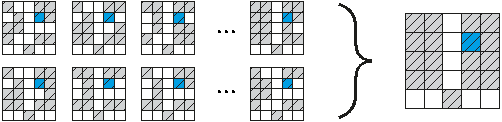
\includegraphics[width=\textwidth]{chapters/understanding-metamaterial-mechanisms-FIG/5-large-search-space.pdf}
    \caption[Short figure name.]{In this example, we have 128 configurations that all lead to the same mechanism, because the cell constraints interact. 
    \label{fig:5-large-search-space}}
\end{figure}

While this example only concerns with one specific scenario, the complete search space would be $2^{25} \approx 3\cdot {10}^7$. We generalize this in Section~\ref{section:search-space} and show how we reduce the search space by several orders of magnitude.


\subsection{Abstract representation reduces the search space}

The key insight of this work is to build an abstract representation of the cell constraints, which defines such distinct mechanisms. We encode constraints that edges impose on each other in a graph whose connected components define their degrees of freedom. We work directly in the reduced space of distinct mechanisms, which are defined by the connected components in the graph, rather than exploring the space of all possible cell configurations. 


\subsection{Computational design tool}

Our constraint-based representation of the metamaterial mechanism and the resulting reduction of the search space makes a computational design tool feasible. We present a computational design tool that optimizes a cell configuration for user-defined paths. Figure \ref{fig:1-editor-walker} shows how users define the size of the mechanism they are looking for and draw the input and output paths. Our heuristic optimization searches for a cell configuration that satisfies these boundary conditions. 


\subsection{Novel types of mechanisms}

With our computational approach, we not only ease the creation process for users, but we also discover new types of mechanical transformations that were not known before. Metamaterial mechanisms were manually designed to demonstrate useful mechanisms, such as a door latch or pliers. However, we show in Figure \ref{fig:6-compare-old-and-new-mechanisms} that the transformations they implemented were basic transformations, such as scaling. In this work, we demonstrate non-linear transformations, as illustrated in Figure 6b, such as self-intersections, oscillations and smoothing. We believe that the approach will foster more complex metamaterial mechanisms. 

\begin{figure} [h]
    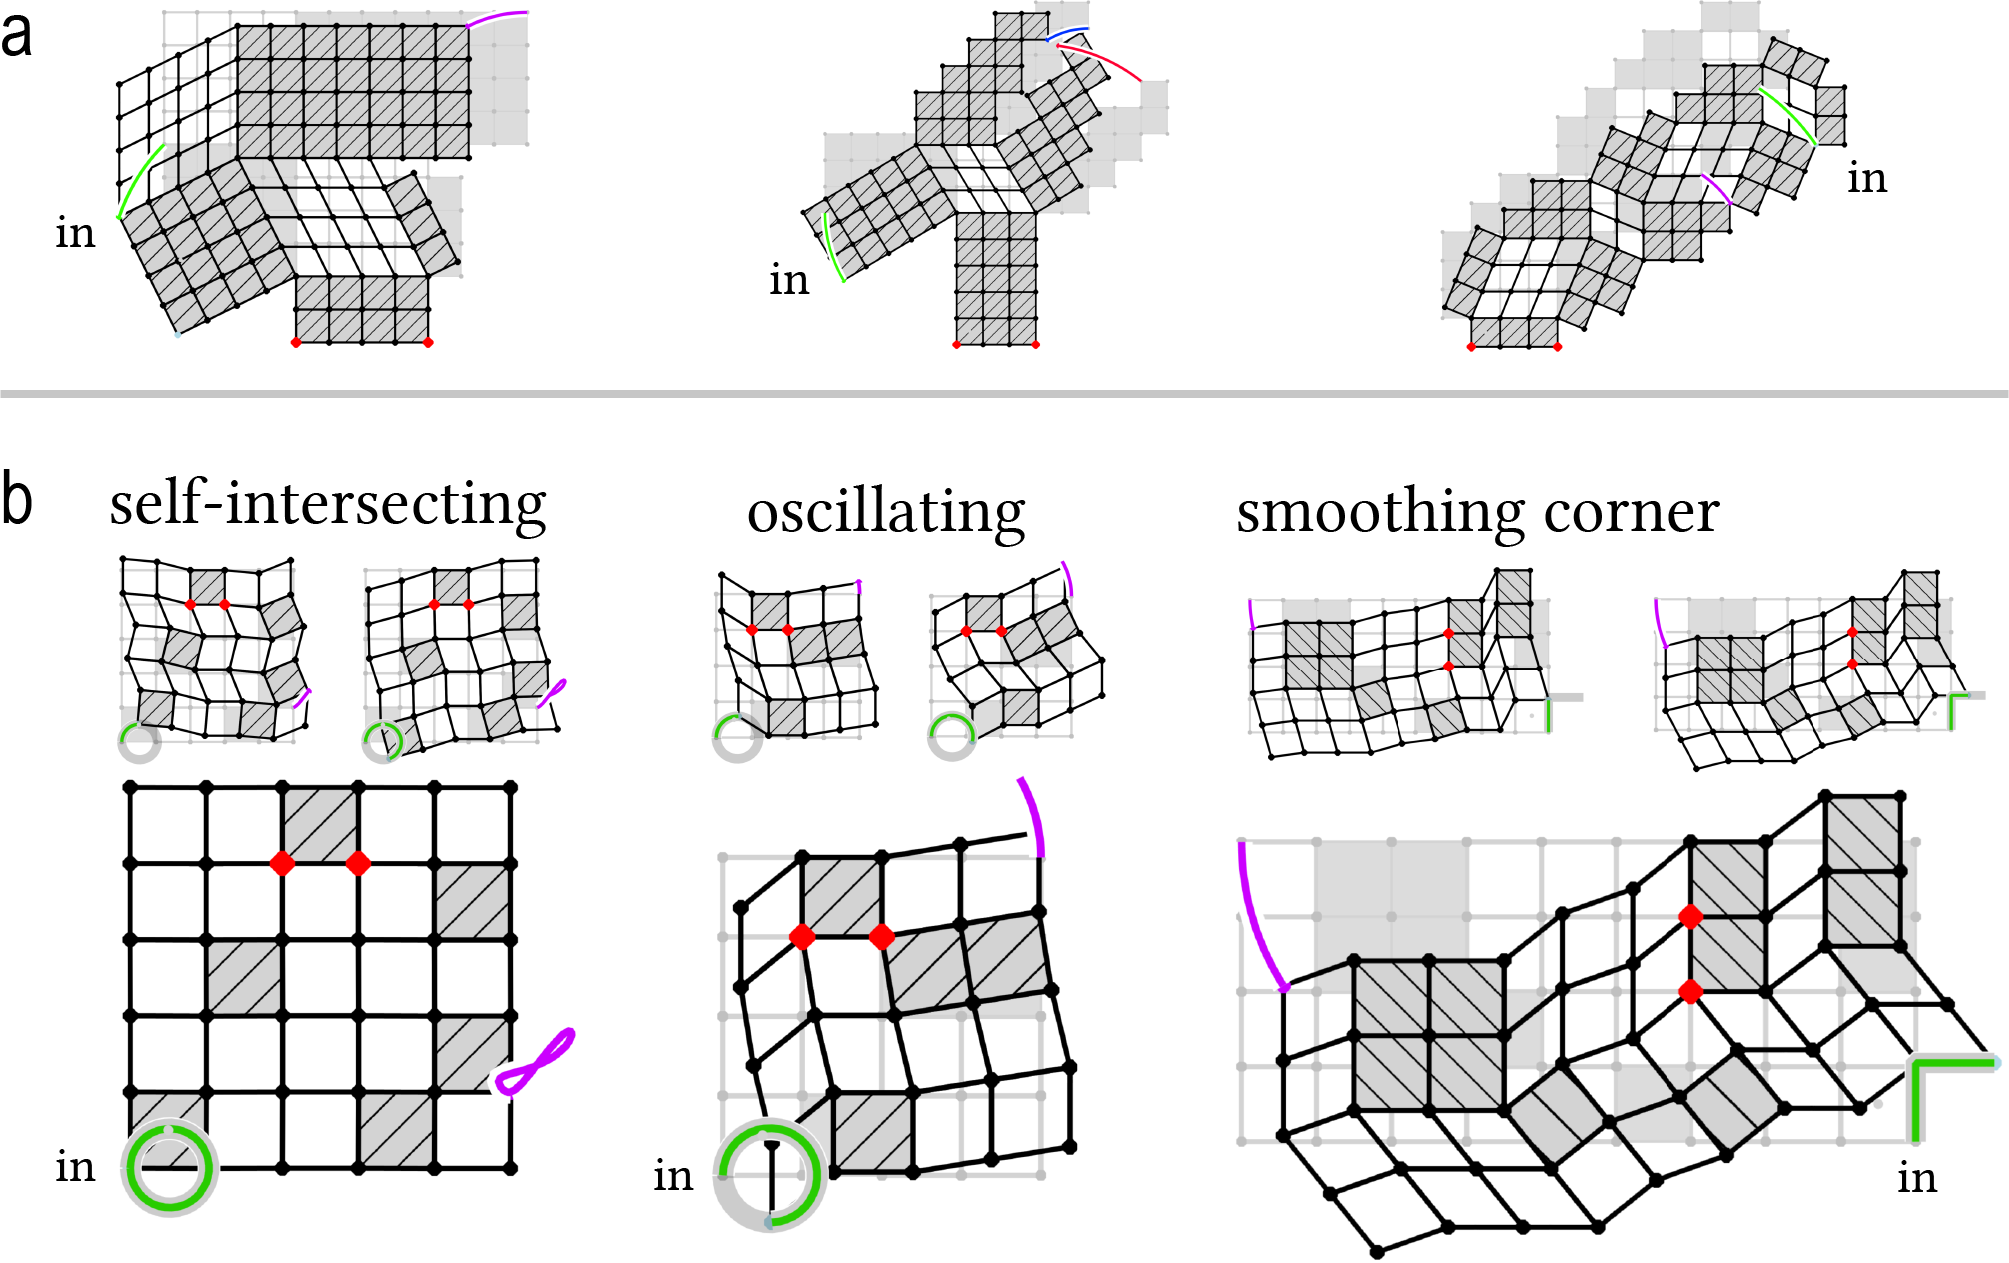
\includegraphics[width=\textwidth]{chapters/understanding-metamaterial-mechanisms-FIG/6-compare-old-and-new-mechanisms.pdf}
    \caption[Short figure name.]{(a) The hand-designed mechanisms in only realize simple transformations. (b) In this work, we discover more complex and even non-linear transformations.
    \label{fig:6-compare-old-and-new-mechanisms}}
\end{figure}


\section{Contributions \& limitations}

Our main contribution is an understanding of the underlying mechanisms of metamaterial mechanisms. Understanding the constraints that interact within a grid enables a computational design tool that would otherwise not have been possible.

While the naive approach of swapping cells on the grid in order to find a cell configuration that implements a user-defined path transformation is computationally infeasible due to an exponentially growing search space, we contribute an abstract representation of the constraints. Our constraint graph representation reduces the search space significantly. 

We show that metamaterials can realize more complex and even non-linear mechanisms---a fact that was unknown before.

However, in this work, we focus on understanding the constraints on the most basic cells, i.e., the square shear and rigid cells. We do not explicitly implement rotated or pre-sheared cells, as suggested in Section~\ref{section:shear-cell}. Since the topology is the same, we show that our constraint graph applied to those cells as well. 


\section{Analysis of cell interactions}

The mechanisms we consider can exhibit intricate behavior even though they are built from very basic building blocks: shearing and rigid cells. Figure \ref{fig:4-constraint-interaction} already demonstrated how drastically a metamaterial can change after performing a small local change, e.g., swapping a shear cell for a rigid cell. These properties are non-obvious but crucial to understand.

In order to understand the movements of a mechanism, we need to simulate its physical behavior numerically. For larger grids the optimization procedure can be time consuming. This can hinder interactive exploration of the space of mechanisms and is especially problematic when sampling and simulating a lot of mechanisms to find one exhibiting some pre-defined behavior.

We describe how we model the constraints of a mechanism, which reduces the number of variables in the physical optimization from all grid points to a few edge vectors. This enables a significantly more efficient implementation and gives insights into the degrees of freedom of a mechanism.


\subsection{Understanding the constraints}
\label{section:graph}

Since our metamaterial consists of shearing and rigid cells, we observe two types of constraints in our cells: (1) parallelism constraints, such that opposing edges always remain parallel and (2) angle constraints, such that angles of rigid cells remain unchanged. Furthermore, all edges maintain their lengths. 
This means most edges cannot move independently, e.g. the same vector can represent edges that have to remain parallel. Edges that have to maintain a certain angle can also be represented by a reference edge that needs to be rotated in order to get the second one. To this end we build a constraint graph in which each node represents a cell edge and an arc between nodes the fact that one edge can be constructed by rotating the other (rotations also include the identity transformation).

Figure \ref{fig:7-single-cell-constraint-graph} illustrates the graph representation for each cell type individually. For shear cells, opposing cell edges always remain parallel. The constraint graph consequently only contains arcs between opposing cell edges. Figure \ref{fig:7-single-cell-constraint-graph}b illustrates that rigid cells are represented by a complete graph. This means that transforming one cell edge defines the transformation of all other edges. In other words, if we know how one edge is, e.g., rotated, we know the transformation of the entire cell, because opposing edges remain parallel and adjacent edges maintain their angle.

\begin{figure} [h]
    \centering
    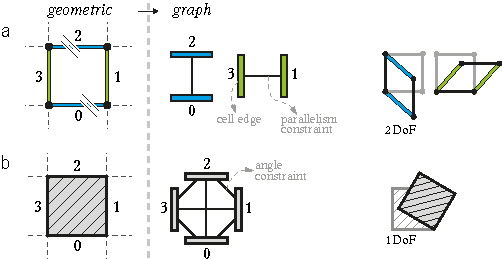
\includegraphics[width=0.95\textwidth]{chapters/understanding-metamaterial-mechanisms-FIG/7-single-cell-constraint-graph.pdf}
    \caption[Short figure name.]{We model the constraints as graphs. (a) A shear cell is represented as 2 subgraphs that model the 2 independently moving adjacent edges and the parallelism constraint of opposing edges. (b) A rigid cell is a complete graph, showing that one edge defined the entire cell.
    \label{fig:7-single-cell-constraint-graph}}
\end{figure}


\subsection{Determining the degrees of freedom}

We think of the degrees of freedom (DoF) as a set of edge vectors that can be transformed independently. This property is also illustrated in Figure \ref{fig:7-single-cell-constraint-graph}, where the constraint graph of the shear cell in (a) consists of 2 connected components, which indicates that the cell has two independently moving parts, i.e., the green and blue edges. The rigid cell in (b) moves as a whole, thus the graph consists of one component. In general, the degrees of freedom of our metamaterial are simply defined by the number of connected components in the constraint graph.


\subsection{Building the constraint graph}

We build the entire constraint graph by connecting the constraints of single cells shown in Figure \ref{fig:7-single-cell-constraint-graph} to their neighbor cells, based on coinciding edges. For example, Figure \ref{fig:8-constraint-graph} shows how to proceed for a metamaterial with 4 cells. We start at the lower left cell and add its vertical edges to the constraint graph. The cell to the right shares the middle vertical edge, thus we link its other vertical edge to the graph, because they need to remain parallel. The two shear cells on the right are processed analogously.  The rigid cell, which cannot change its angle, effectively couples edges of the top right and lower left cell. Due to the parallelism constraints, entire rows and columns are linked. 

\begin{figure} [h]
    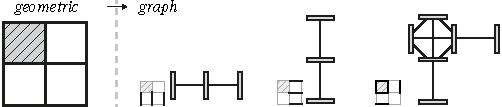
\includegraphics[width=\textwidth]{chapters/understanding-metamaterial-mechanisms-FIG/8-constraint-graph.pdf}
    \caption[Short figure name.]{We build the constraint graph by connecting the single cell constraints to their neighbor cells based on coinciding edges. 
    \label{fig:8-constraint-graph}}
\end{figure}

The notion of degree of freedom generalizes to entire mechanisms. The final graph in our example consists of 3 connected components, which tells us that the configuration has 3 DoF. Knowing one edge vector in each component uniquely determines all other edge vectors and thereby the whole mechanism. Therefore, we can formulate an optimization problem only involving 3 instead of 12 edges. We will provide details on this idea in Section~\ref{section:optimization}. 

In a cell grid that consists only of shear cells, the edges in each row and column represent one connected component each. The maximal number of degrees of freedom on an empty $n \times m$ grid is therefore $n+m$. Introducing a rigid cell joins the components of a row and a column into one, reducing the number of degrees of freedom by one.


\subsection{The influence of anchors}

So far, we only considered relative transformations of edges, i.e., edges are transformed with respect to each other. However, since the input of a mechanism is absolute, we need to fixate (i.e., anchor) the cell configuration in order to calculate the vertex positions in absolute space. 

Anchoring an edge in a cell configuration reduces its degrees of freedom by one. The same reasoning as for transforming edges, as discussed above, applies; since one edge of a connected component is defined (here, fixed to the ground), all edges in the component are defined. Furthermore, anchors define the scaling of an output path. As shown in Figure \ref{fig:9-anchor-effects}a, the length of the target paths is proportional to the distance between the anchors and the target vertices. Figure \ref{fig:9-anchor-effects}b illustrates, that anchors define a global rotation point.

\begin{figure} [h]
    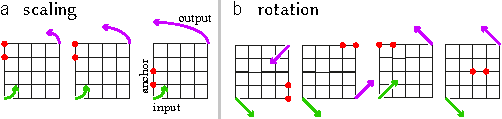
\includegraphics[width=\textwidth]{chapters/understanding-metamaterial-mechanisms-FIG/9-anchor-effects.pdf}
    \caption[Short figure name.]{The anchor placement influences (a) the scaling of the output path and (b) the global rotation. 
    \label{fig:9-anchor-effects}}
\end{figure}


\section{Reducing the search space}
\label{section:search-space}

Since each cell on a $n\times m$ grid can have 2 states, rigid or shearing, we have $2^{nm}$ different possible configurations. However, not all configurations will generate a unique mechanism since shearing cells can become rigid because of the constraints. Consider the mechanism in Figure \ref{fig:10-non-shearing-constraint-graph}. The constraint graph reveals that the green and blue cells cannot shear. This is the case when \textit{all edges} of a cell are contained in the \textit{same connected component}. Since the rotation of both potentially independent edges of the shear cell are defined by the same connected component, their angle is constraint to the original 90° and can thus not shear.

\begin{figure} [h]
    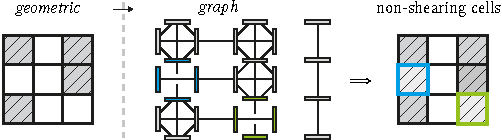
\includegraphics[width=\textwidth]{chapters/understanding-metamaterial-mechanisms-FIG/10-non-shearing-constraint-graph.pdf}
    \caption[Short figure name.]{It might be non-obvious how many DoF this metamaterial has. Our constraint graph reveals that it contains 2 cells that cannot shear, i.e., the blue and the green one, leaving only 2 DoF.
    \label{fig:10-non-shearing-constraint-graph}}
\end{figure}

Since the blue and green cells cannot shear, the two cell configurations in Figure \ref{fig:10-non-shearing-constraint-graph} are equivalent. We only want to consider \textit{unique mechanisms} in our optimization. But how many of these unique mechanisms exist? To answer this question, we enumerate all possible connected component configurations. It is indeed possible to give an explicit formula for the number of all unique mechanisms on a $n \times m$ grid. 
We present the derivation of this function in Appendix \ref{appendix:unique-mechanisms}. Here, we show the empirical verification the formula for all configurations on grids with $n<5$. 
In Figure \ref{fig:11-search-space-reduction}, we show the number of all $2^{nn}$ mechanisms (gray) along with the number of unique mechanisms (blue). While this number still grows rapidly with increasing grid size it reduces the space of configurations on a grid from growing quadratically with respect to n in the log-plot to linearly, which is already significantly better. This enables us to consider much larger grids when searching for mechanisms with certain properties. 

\begin{figure} [h]
    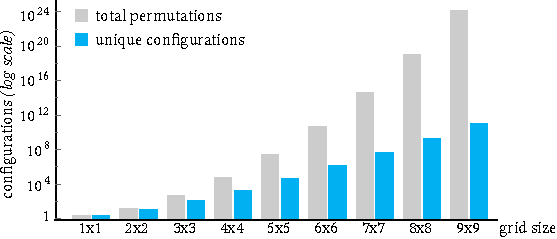
\includegraphics[width=\textwidth]{chapters/understanding-metamaterial-mechanisms-FIG/11-search-space-reduction.pdf}
    \caption[Short figure name.]{The number of all configurations (log scale) on a square grid com-pared to the number of all unique mechanisms. 
    \label{fig:11-search-space-reduction}}
\end{figure}


\section{Simulating the motion}
\label{section:simulation}

To simulate the deformation of the object when a vertex of a cell moves, we use a simple elastic material model. We assume the edges are rigid and deformation occurs when two edges incident to a corner are rotated relative to each other. 

Through the constraint graph all edges are defined as soon as one representative edge per connected component is known. To define the remaining edges, we traverse the constraint graph, e.g. using breadth-first search, starting at the representative edge. When moving across an arc the appropriate rotation is applied. When all edges are known we can start to reconstruct cell vertices. To this end we traverse the grid itself starting at an anchored vertex. Each vertex is effectively reconstructed by summing all edge vectors along a path connecting the vertex to the anchor. 

Direct numerical simulation would try to find a set of grid vertices minimizing this deformation energy subject to a set of non-linear constraints, edges have to maintain their length, opposing edges in a cell have to stay parallel and angles in rigid cells stay at 90°. Additionally, certain vertices are fixed, either in their original position or by an external force driving the mechanism. 

Analyzing the constraint graph allows us to formulate a constrained optimization problem that has the same solution but is much more efficient than the direct approach.

The shape of the whole mechanism is determined by fixing the degrees of freedom, which requires two numbers per connected component. The current state of the deformation can therefore be modeled by a state vector $x\in\mathbb{R}^{2\ N_d}$ where $\ N_d$ is the number of degrees of freedom. Each state vector uniquely determines all edge vectors and is associated with the deformation energy

$$ D\left(x\right)=\sum_{i=0}^{N-1}\left(\alpha_i\left(x\right)-\frac{\pi}{2}\right)^2,$$

where $\alpha_i(x)$ stand for an interior angle of the i-th cell and $N$ for the number of cells. This energy models the fact that each cell will, depending on the material used, resist shearing, even for non-rigid cells. Note, that we only need to take one angle per cell into account because all angles in a cell produce the same energy. 

To simulate the deformation, we find a minimizer of $D$ with respect to the following constraints:

\begin{itemize}
	\item [C1.] The edges are rigid and therefore have to be fixed in length. Constraining all degrees of freedom to unit length will ensure this property for all edges in the mechanism.
	\item [C2.] Cells cannot invert, i.e., change their orientation. We therefore assure that the cell areas always remain positive.
	\item [C3.] Anchors are fixed in position.
    \item [C4.] The corner that is being dragged is fixed in position.
\end{itemize}
    
Note that we do not have to enforce that edges are parallel in shear cells or that rigid cells maintain their interior angles. These constraints are already built into the reduced representation and each state vector induces a valid cell layout. This constitutes another advantage over the direct approach where these constraints have to be taken into account explicitly.

Unfortunately, the energy and the constraints are non-linear and non-convex. However, the constraints are only quadratic and they can be analytically differentiated. The energy $D$ can also be analytically differentiated albeit yielding more complex terms due to the calculation of angles from edge vectors.
We solve the problem of minimizing $D$ subject to C1-C4 by employing the non-linear interior point solver IPOPT \cite{Waechter2006}, which gives us a configuration for a specific handle position. To simulate the full deformation, we sample the desired handle path and find the correct configuration by solving the optimization problem starting from the previous configuration as an initial guess.


\subsection{Invalid input}

The range of the handle corner is limited by the structure of the mechanism, which is fixed by anchors. If a handle position outside this range is prescribed the optimization problem has no solution because C4 cannot be satisfied. To yield an approximate result even for these situations we try to find a handle position, which is close to the desired one but in the range of the handle. To this end we solve another optimization problem minimizing the distance of the updated handle position ${\widetilde{P}}_h$ to the prescribed one $P_h$:

$$D\prime \left(x\right)=\left \| {\widetilde{P}}_h-P_h \right \|^2,$$

subject to the constraints C1-C3. The resulting configuration is one that is valid and places the handle close to the desired position. However, the solution represents only one valid configuration, which will not minimize $D$ in general. We therefore optimize $D$ with respect to C1-C4 using the new handle constraint.


\subsubsection{Evaluation}

As a preliminary evaluation of the simulation, we manually created 3 mechanisms with different inputs in our software and manufactured them from laser cut acrylic and 3D printed hinges (Ninjaflex filament). We tracked the motion of the physical mechanisms using OptiTrack with up to 7 markers on each mechanism and compared it with motion paths from our simulation. We adjusted the OptiTrack data to account for scaling. Figure \ref{fig:12-optitrack-evaluation} shows at one example that the recorded and simulated data matched closely. These experiments support that the results of our simulation match the behavior of physical mechanisms.

\begin{figure} [h]
    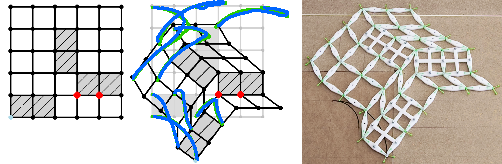
\includegraphics[width=\textwidth]{chapters/understanding-metamaterial-mechanisms-FIG/12-optitrack-evaluation.pdf}
    \caption[Short figure name.]{Example of our evaluation. The green path represents the paths from our simulation, blue is the data from OptiTrack.
    \label{fig:12-optitrack-evaluation}}
\end{figure}


\section{Optimization of cell patterns}
\label{section:optimization}

We aim to alleviate the problem of finding suitable configuration of cells given a set of desired input and output paths. In the following, we detail our algorithm that exploits aforementioned properties of metamaterials mechanisms such as the relation between cell transformation and anchors, and the constraint graph. Note that while most of our examples illustrate quadratic cell configurations, the approach is equally applicable for arbitrarily shaped objects. The main requirement for our approach is a simulation that correctly reproduces the deformation of a mechanism given an input path, like the one described in the previous section.

\subsection{Overview}

Our algorithm takes a set of user-defined input and output paths as well as a rough shape of the desired device as input. Our algorithm aims to find a close-to-optimal fit between the motion of the mechanism and the user-defined paths. Generally, input paths are actuated (e.g., by users) and the mechanism transforms this motion to the output path. In context of the optimization, however, we do not need to differentiate between input and output paths but use them as a list of paths which a mechanism should be able to reproduce. As a first step in our algorithm, we automatically determine the positions of the anchors for the cell configuration based on the scale and direction of the paths. We then generate a mechanism that produces the desired motion. An overview of the algorithm is illustrated in Figure \ref{fig:13-optimization-overview}.

\begin{figure} [!h]
    \centering
    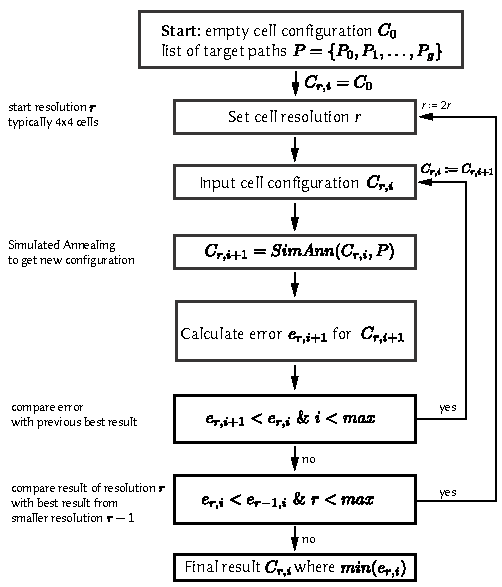
\includegraphics[width=\textwidth]{chapters/understanding-metamaterial-mechanisms-FIG/13-optimization-overview.pdf}
    \caption[Short figure name.]{Overview of the process of automatically finding cell patterns given user-specified paths.
    \label{fig:13-optimization-overview}}
\end{figure}

Since the behavior of a mechanism is non-linear, we create cell configurations using stochastic optimization, specifically Simulated Annealing \cite{Ram1996, Kirkpatrick1983}. Instead of modifying the cell configuration directly, we modify the constraint graph, i.e., split and merge connected components until the algorithm converges. To speed up computation, we resort to a hierarchical approach where we first find an optimum configuration for scaled-down versions of the mechanism and use this configuration as seed for larger versions. The output of the algorithm is a cell configuration that produces the desired paths.


\subsection{Input and representation}

Users specify the shape of the cell configuration, denoted as $C_0\in{0,1}^{x,y}$, with $x$ and $y$ being the dimensions of the mechanism. This is a configuration of cells with undefined behavior. In the later optimization, the type of each cell is specified (e.g., they become shear or rigid cells), which ultimately governs the motion of the mechanism. Each mechanism is by its cells and its vertices $V$ and edges $E$. The position of the anchors $A\subseteq V$ governs the motion of a mechanism and fixes the mechanisms absolute position in space. Anchors are automatically determined by our algorithm.

Besides $C_0$, users specify a set of desired paths $P={P_0,\ P_1,\ldots,\ P_m}$. Each path is a list of points, stored as matrix $P_i\in\mathbb{R}^{2\times n}$. The first point $p_{i,0}$ of a path $P_i$ is a vertex of the cell configuration, i.e.,  $p_{i,0}\in V$. Note that while we use one input and one output path for clarity of exposure, the optimization generalizes to more than one input and output path.


\subsection{Setting anchors}

Our algorithm automatically determines candidates for positions of the anchors based on user-defined paths. This is done by anchoring a single edge $e$ (i.e., setting its two vertices to be anchors). There are three main considerations that govern the positioning of the anchors (i.e., finding which edge to anchor). First, the ratio between the length of paths should be similar to the ratio between the distance between individual paths and the anchors. As an example, if an input path is half the length of an output path (i.e., scale ratio 1:2), then the ratio for the distance between input path and anchors, and the output path and anchors should be similar. This accounts for scaling between the paths and can be calculated as

$$\min_l
{
\sum_{i=0}^{m}
\sum_{j=i+1}^{m}
{\frac{\left| P_i \right|}{\left| P_j \right|}}
-
{\frac{\left| e_l-P_i \right|}{\left| e_l-P_j \right|}}
}
$$

where $m$ denotes the number of user-defined paths. Secondly, anchors are essentially rotation points between paths. We therefore choose the location of anchors to reflect this rotation. Thirdly, to allow for maximum motion range of a path, the anchors should be as far ways from all path points as possible. This is formulated as 

$$\max_l{\sum_{i=0}^{s}\left|e_l-P_i\right|.}$$

Since this operation can be performed on a scale-down version of the configuration, we can exhaustively search the space and choose the best anchor positions. It is possible that no valid positions are found, e.g., if the length of a path exceeds to overall diagonal length of the cell configuration. If this is the case, users can adjust the paths, e.g., decrease the overall length of the paths.


\subsection{Generation of cell configurations}

Given a list of user-defined paths, any cell configuration $C$ will transform the paths in a specific way. For a single path $P_i$, this transformation is denoted as $C\left(P_i\right)$. We aim at finding a cell configuration $C_j$ with the minimal difference between $P_i$ and $C\left(P_i\right)$ while using as few as possible degrees of freedom to increase mechanical stability. We thus aim to find a solution (i.e., a close-to-optimal cell configuration) given the objective

$$\min_j{\sum_{i=0}^{m}{\omega_i \left| P_i-C_j \left( P_i \right) \right|.}}$$

$\omega_i\in\left[0,1\right],\ \ \sum_{i=0}^{m} \omega_i \mathrel{\mathop:}= 1$ 
are user-defined weighting factor for the individual paths. In our implementation, we typically use equal weights for input and output path (i.e., 0.5 for 2 paths).

A trivial approach to the problem would be to randomly sample cell configurations (i.e., switching cell types randomly) and choose the best fit between the user-defined paths and the paths the mechanism produces. This, however, is not feasible, as discussed in Section~\ref{section:search-space}, given the large number of possible cell configurations that yield similar movements or are rigid. 

In our approach, instead of modifying the cell configuration directly, we manipulate the underlying constraint graph with respect to the degrees of freedom of a configuration. We typically aim for a configuration with as little degrees of freedom as possible that still can reproduce a path well. A too low number of degrees of freedom would not allow for complex motion (e.g., with changes in direction). A too high number of degrees of freedom would lead to mechanically unstable structures. Therefore, we constrain a configuration to be within ${DoF}_{min}$ and ${DoF}_{max}$, which are typically chosen to be 2 and 5, respectively. 

For each step in our optimization, we compute the current degrees of freedom ${DoF}_j$ for a configuration $C_j$. The degrees of freedom govern the next step, i.e., if the next configuration shall contain more or less degrees of freedom. If the degrees of freedom should be increased, we split a chosen connected component. Conversely, we merge two connected components to decrease the degrees of freedom. If the degrees of freedom are within the limits, an operation is chosen randomly. The connected components that are affected by the operation are chosen randomly. 

We use Simulated Annealing for the optimization to avoid converging to a local minimum. We calculate the current temperature $T_j$ for each step as

$$T_k=(1+e^\frac{e_k}{T_0\alpha^k})^{-1},$$

where $e_k$ denotes the error of the current iteration $k$. It is calculated with respect the overall objects as the sum of differences between as user-defined paths, i.e. $e_k=\sum_{i=0}^{m}{\omega_i\left|P_i-C_k\left(P_i\right)\right|.}$ The error is normalized with respect to the length of the paths. $T_0$ is the starting temperature, which we typically choose as one third of the number of maximum iterations, as described below. $\alpha$ control the overall falloff of the algorithm, typically $0.85 < \alpha < 0.99$ (in our case, we chose $\alpha$ as $0.95$). To avoid that the algorithm converges in a local minimum, we restart the Simulated Annealing process several times. After each run, we compare the best results of the current and previous run. Converges is reached if the result did not improve compared to the previous run.


\subsubsection{Hierarchical generation}

We chose a hierarchical approach for the optimization, to avoid users having to estimate the cell resolution of their configuration. We start the Simulated Annealing process for an initial configuration $C_0$ with a small resolution r, e.g., 4 $\times$ 4 cells. Once the previously described Simulated Annealing procedure converged, we double the resolution and restart the Simulated Annealing with the larger resolution $r+1$. After convergence, we compare the error of the cell configuration $C_r$ and $C_{r+1}$. In case the result did not improve, we assume $C_r$ to be the best solution. If the result did improve, we increase the resolution again and restart the process. A typical error function for the whole process is shown in Figure \ref{fig:14-optimization-error-analysis}. Since the process typically converged after 100 to 150 iterations, we set the number of maximum iterations to 200. Similarly, the algorithm typically converges after increasing the resolution 2 to 3 times. We therefore set the maximum number of increasing the resolution to 5.

\begin{figure} [h]
    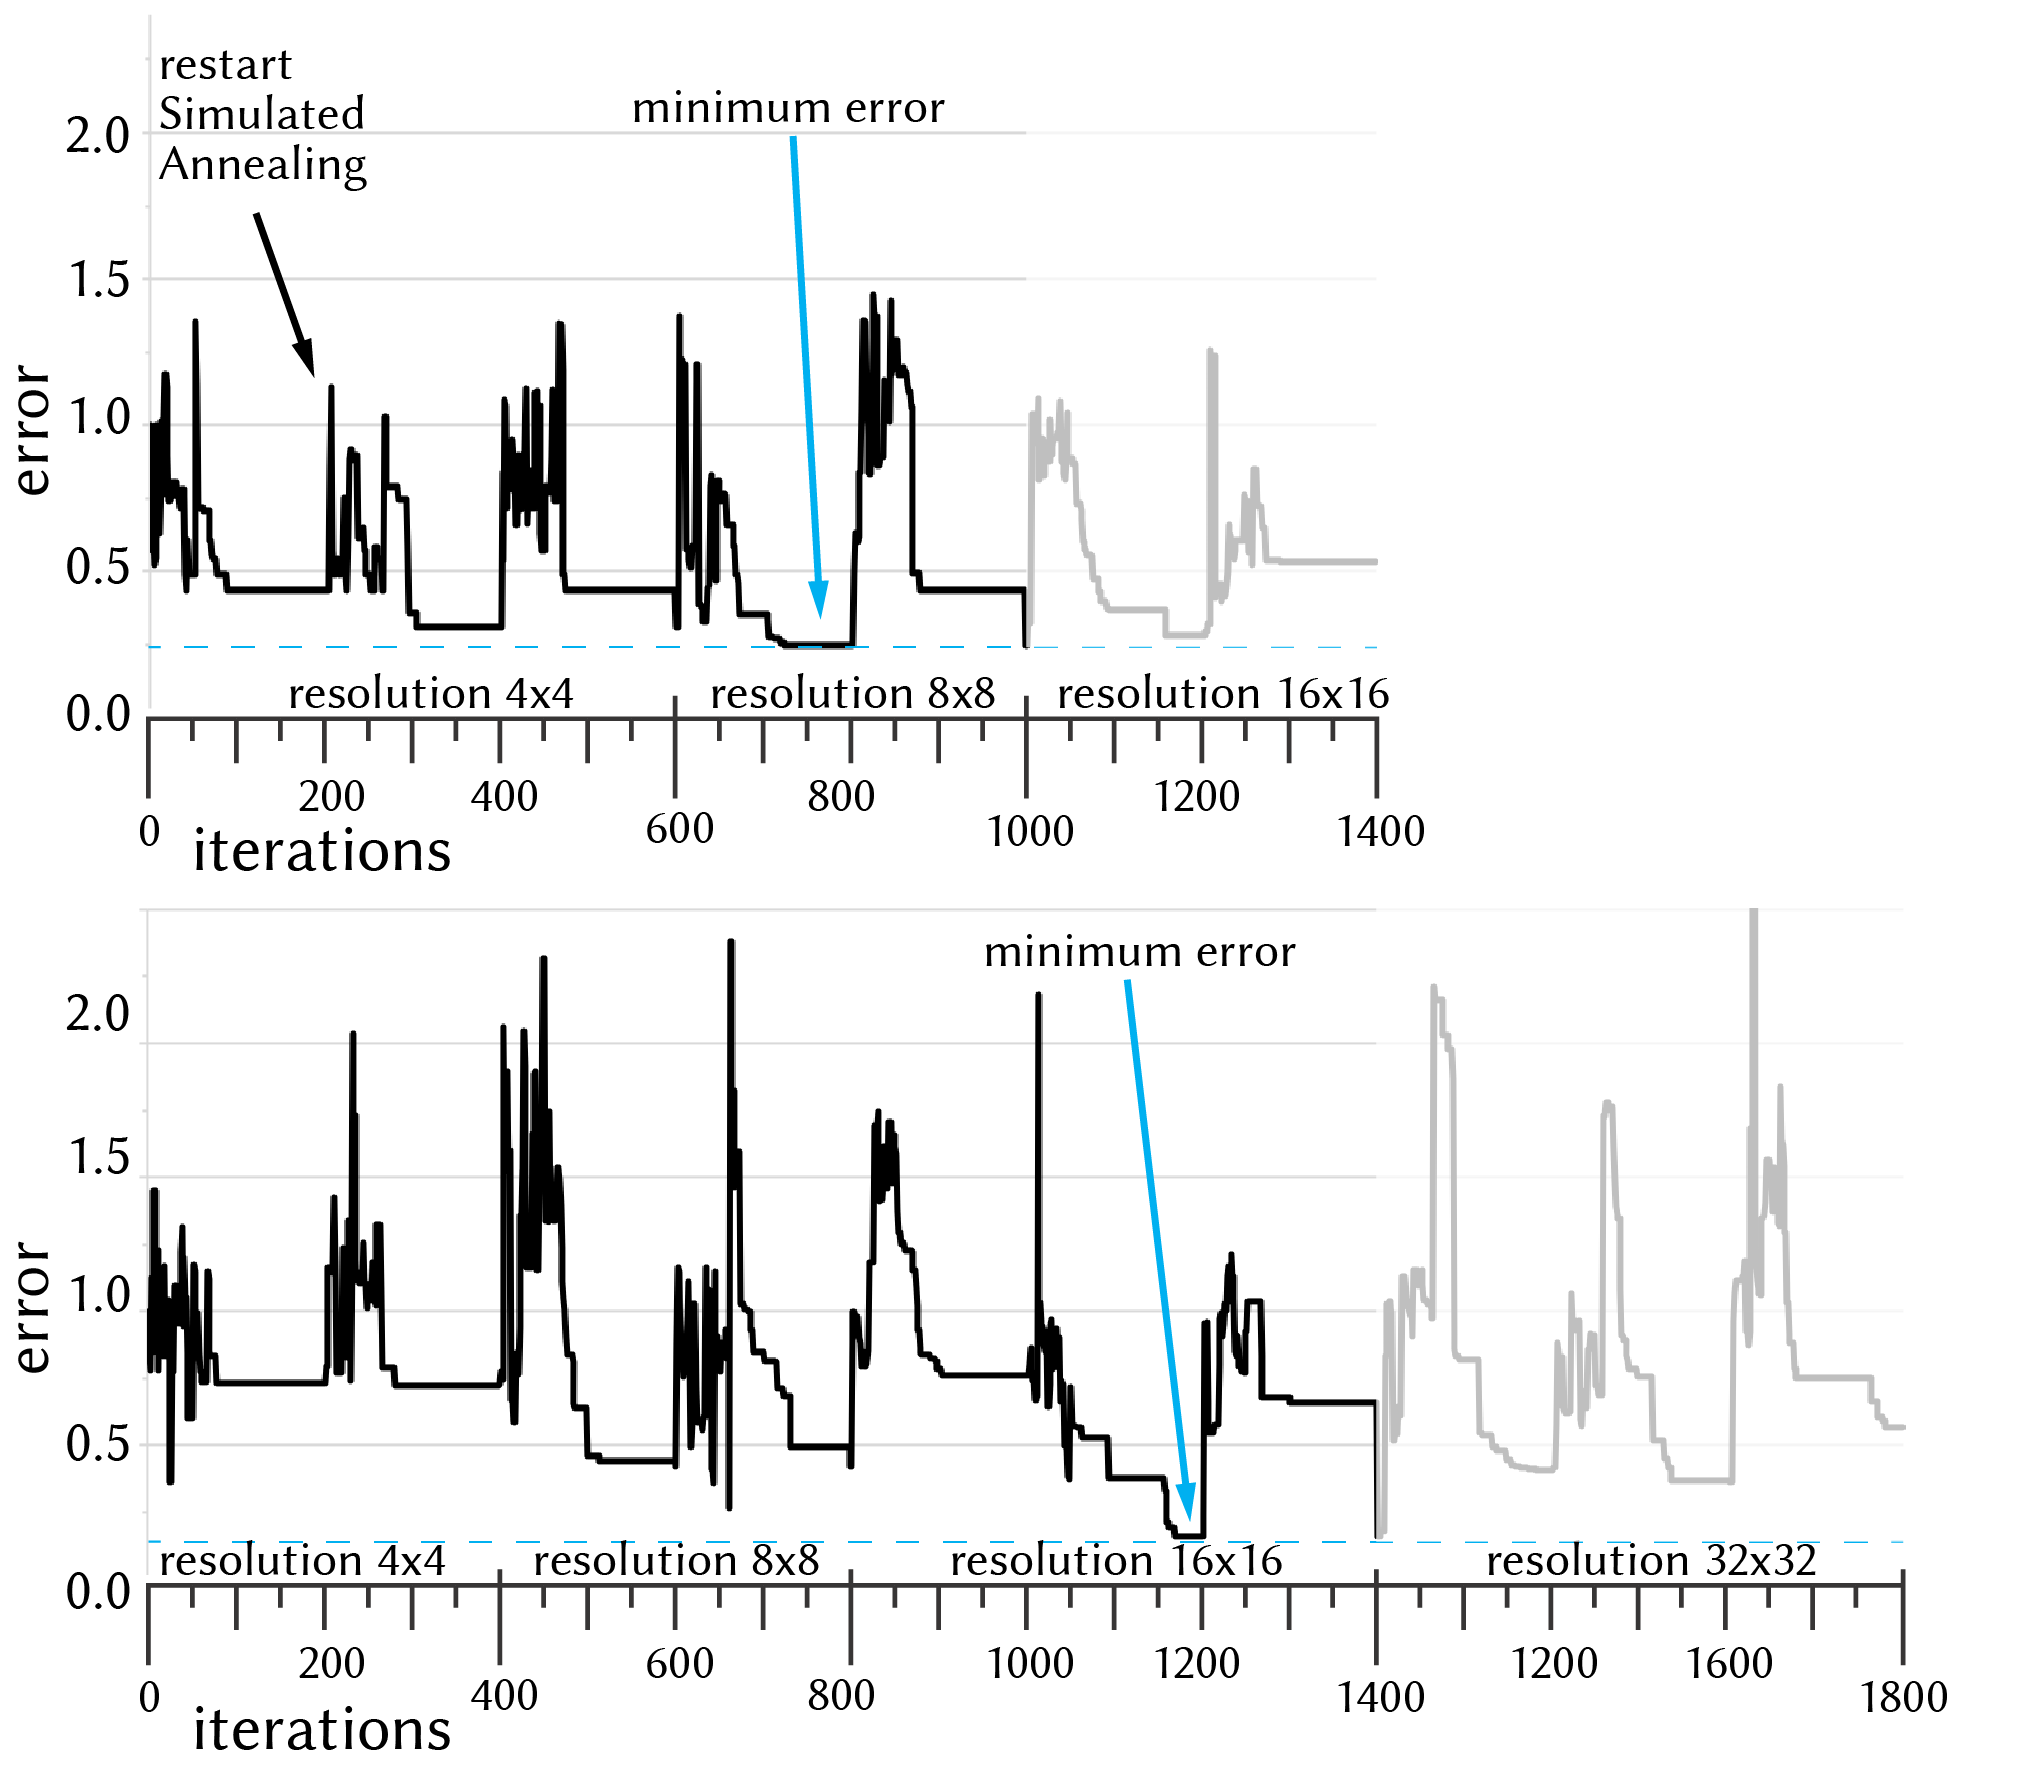
\includegraphics[width=\textwidth]{chapters/understanding-metamaterial-mechanisms-FIG/14-optimization-error-analysis.png}
    \caption[Short figure name.]{Typical error function for two examples. For top, the process con-verged after a total of 1400 iterations, with the minimum error for a resolution of 8 $\times$ 8 cells. Results with higher resolution (16 $\times$ 16) were discarded due to increased error. The bottom example converged with a resolution of 16 $\times$ 16 cells. For each resolution, Simulated Annealing is restarted multiple times.
    \label{fig:14-optimization-error-analysis}}
\end{figure}


\subsection{Evaluation}

We randomized a small number of ground truth examples to evaluate if the optimization finds an optimal solution given a user-defined input and output path. We randomly generated 10 cell configurations with 3 or 4 degrees of freedom. We manually set the input and output vertex, an input path and the anchors. Inputting this into the simulation yielded an output path. The input path and output path, as well as an empty low-resolution cell configuration with correct aspect ratio were given as input for the optimization. The resulting cell configurations, although different in terms of cell configuration and anchoring, could all truthfully reproduce the target movement. Two examples with target and solution are shown in Figure \ref{fig:15-groundtruth-test}. 

Note that the cell configuration, the anchors and the target resolution were not known to the optimization but were generated.

\begin{figure} [h]
    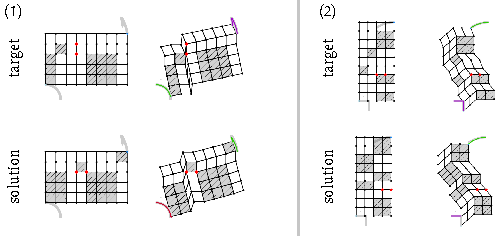
\includegraphics[width=\textwidth]{chapters/understanding-metamaterial-mechanisms-FIG/15-groundtruth-test.pdf}
    \caption[Short figure name.]{Two of ten ground truth examples (top) we used to test the optimization. The results in the bottom were generated without inputting the cell configuration or position of the anchors into the optimization procedure.
    \label{fig:15-groundtruth-test}}
\end{figure}


\subsection{Implementation}

While we already discussed the optimization and simulation in previous sections, we want to briefly mention the frameworks we used. We packed the metamaterial mechanism optimization, as described above, into a simple editor. The editor allows users to draw the shape of their desired mechanism and to set input and output paths, which the software will optimize for. Users can use pre-defined paths for precise motion constraints or simply draw rough paths. Time needed to generate a cell configuration depends on whether the solution requires a high-resolution configuration. If the solution is found in a low-resolution grid, the algorithm takes approximately 1 minute to converge on a commodity notebook (MacBook Pro 2015 with Bootcamp). For higher resolutions (e.g., 32 $\times$ 32 cells), finding the best solution takes up to 10 minutes. We are confident that we this time can be decreased by parallelizing parts of the algorithm, e.g., running multiple threads of Simulated Annealing at once. The editor is implemented in C\# and uses the .NET framework 4.5. We use the Windows Presentation Foundation (WPF) as our GUI toolkit. The optimization procedure is also implemented in C\#, which calls a wrapper to our C++ simulation tool. The simulation is written in C++, because it uses IPOPT \cite{Waechter2006}, as we discussed in Section~\ref{section:simulation}. We will provide the source code prior to the conference.

\subsection{Limitations of the design tool}

The editing capabilities of our editor are currently limited to 2D. Furthermore, we implemented only square cells so far. Triangular, rotated, or pre-sheared cells, as suggested in Section~\ref{section:shear-cell} are not integrated in the current version of the editor. However, this would be a simple extension.  We also currently don’t offer mesh export options, as we focused on the optimization. A conceivable option would be to implement the tool as a plugin to existing CAD tools, e.g., Autodesk Fusion 360, as they offer elaborate modeling options for the parts that embed the metamaterial.


\section{Examples}

The main contribution of this work is the abstract representation of metamaterial mechanisms, which ultimately allows an automatic generation of such metamaterials. While the device that embeds the metamaterial is not the focus of this work, we want to give some brief examples of how our generated metamaterials might be embedded in a device-context. This work allows to create new types of mechanisms, which experts of mechanism design can add to their repertoire. The examples here are merely intended to foster future discussion and research of monolithic cell-based mechanisms. More transformations are listed as examples in Appendix \ref{appendix:example-transformations}.

\paragraph{Kinetic sculptures.} One example, where metamaterial mechanisms might be embedded into, are kinetic sculptures, toys, or walking automata \cite{Thomaszewski2014}. As shown in Figure \ref{fig:16-examples-walker}, our design tool enables users to create custom walk-cycles from metamaterials. 

\begin{figure} [h!]
    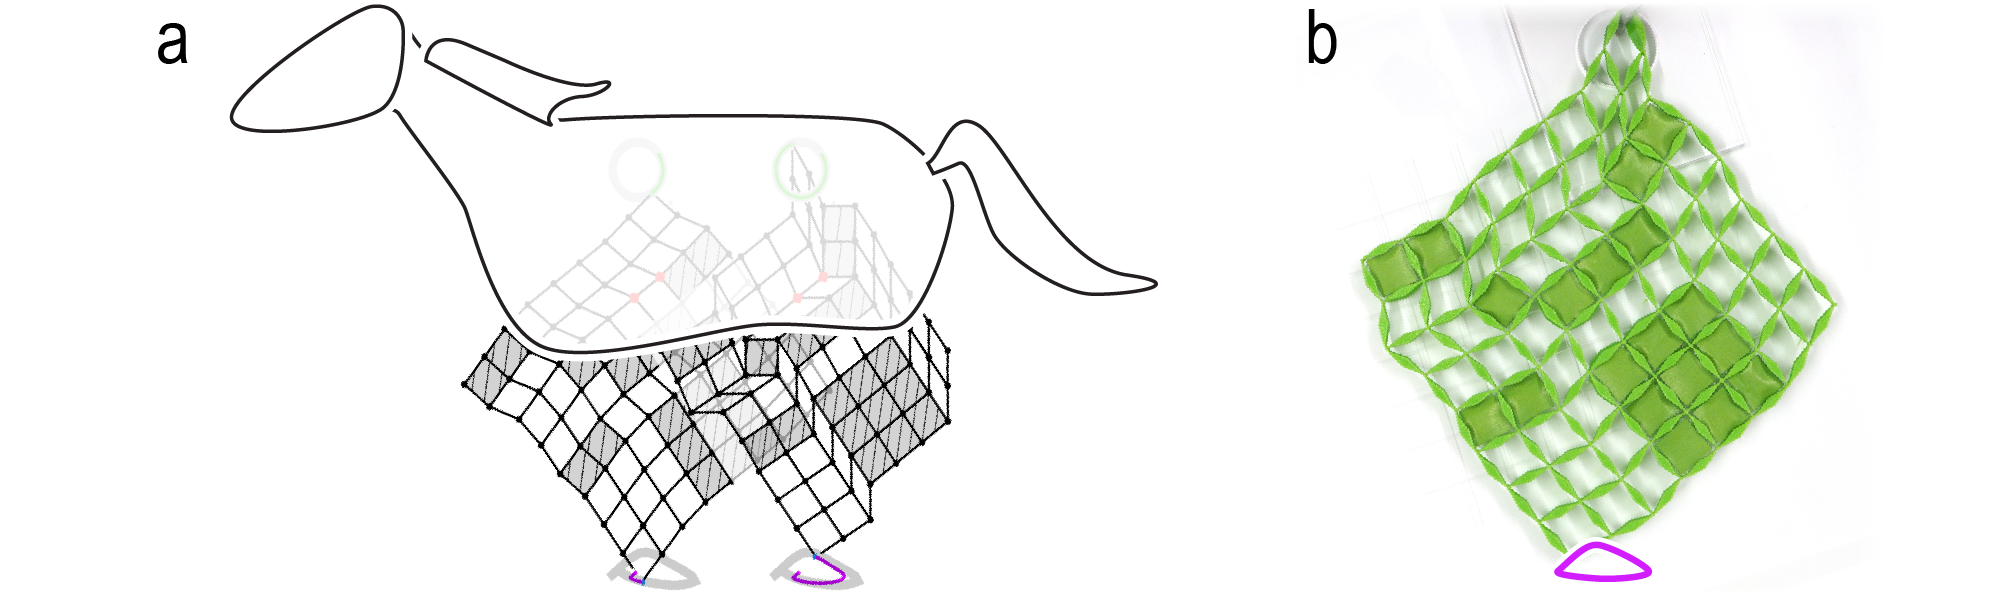
\includegraphics[width=\textwidth]{chapters/understanding-metamaterial-mechanisms-FIG/16-examples-walker.pdf}
    \caption[Short figure name.]{Embedding metamaterial mechanisms into kinetic sculptures. 
    \label{fig:16-examples-walker}}
\end{figure}

\paragraph{Custom mechanisms.} Users might also want to create grippers with a custom motion path. In Figure \ref{fig:17-examples-gripper}, we illustrate embedding metamaterial mechanisms with different motion paths as grippers for collecting items, e.g., for picking-challenge robots. Other applications for such custom paths that come to mind are, e.g., fans with a path cycle, or deflectors for sprinkler which can be customized to sprinkle a specific area optimally.

\begin{figure} [h!]
    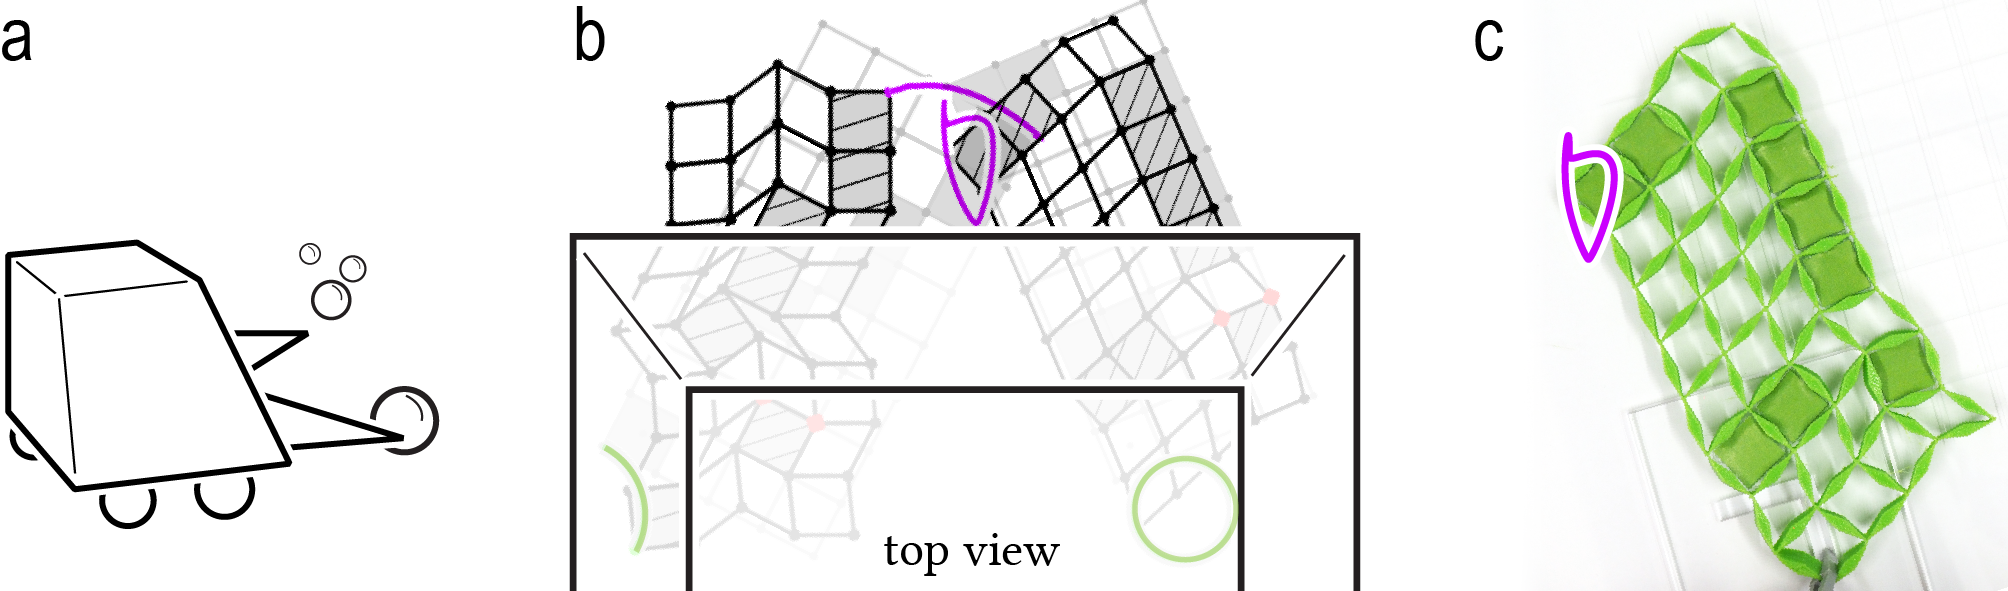
\includegraphics[width=\textwidth]{chapters/understanding-metamaterial-mechanisms-FIG/17-examples-gripper.pdf}
    \caption[Short figure name.]{Example of metamaterial mechanisms as gripper with custom motions for, e.g., robots.
    \label{fig:17-examples-gripper}}
\end{figure}

\paragraph{Clock.} Another simple example is an alarm clock, as depicted in Figure \ref{fig:18-examples-oscillating-clock}. The metamaterial transforms a rotary input into an oscillating motion to strike the bells.

\begin{figure} [h!]
    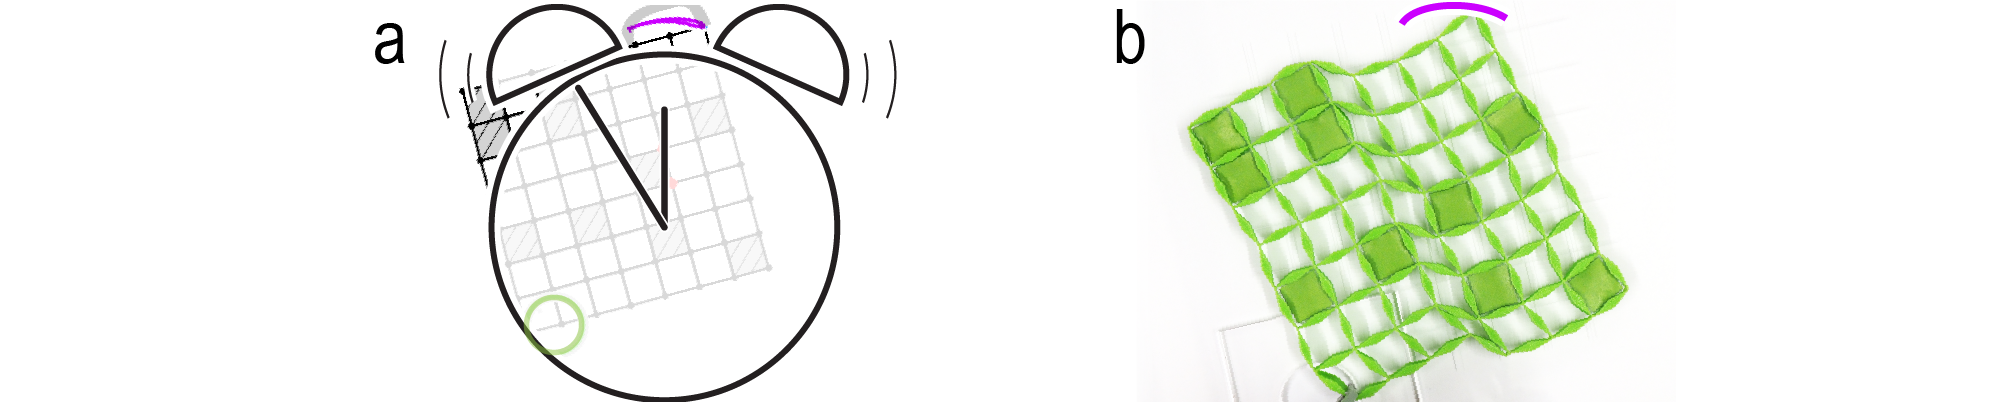
\includegraphics[width=\textwidth]{chapters/understanding-metamaterial-mechanisms-FIG/18-examples-oscillating-clock.pdf}
    \caption[Short figure name.]{A simple example is embedding an oscillating metamaterial into an alarm clock.
    \label{fig:18-examples-oscillating-clock}}
\end{figure}


\section{Discussion \& outlook}

Our work aims at providing an understanding of metamaterial mechanisms and go beyond purely exploratory work. Our work opens way for researchers to explore, build and use such mechanisms. Moving away from a representation that is based on cells to a higher level---the constraint graph---allowed us to significantly reduce the space of cell configurations, making computational approaches feasible. Note that while the search space is highly reduced, it is still not feasible to fully enumerate the space. As discussed above, a cell configuration of 9 $\times$ 9 cells yields $10^{12}$ unique transformations (but $10^{24}$ cell configurations). We are confident, however, that our work informs the research in the space and can provide a foundation to make metamaterial mechanisms accessible to a broader audience. 


\subsection{Limitations and considerations}

The constraints graph and the optimization allow us to generate insights into the inner workings of metamaterial mechanisms and create a computational tool that allows for their automatic generation. There are, however, limitations to our approach.

\subsubsection{Transformation symmetry}
For a given cell configuration, moving an input vertex along the input path yields a transformation of the output vertex, resulting in an output path. If, however, the output vertex is moved along the same output path, the transformation of the input vertex is not equal to the input path. This behavior has to be taken into account when designing mechanisms that should be actuated from by moving the input and the output vertex. It can, however, also be exploited to create more interesting and complex mechanisms.

\subsubsection{Transformation complexity}
In our experiments, we observed that transformation between an input and an output path are limited in their complexity. Specifically, we saw that the number of inflection points between the two paths is roughly the same. An input path with one inflection points, for example, usually yields output paths with zero to two inflection points, but not arbitrary number. 

\subsubsection{Error cases of the optimization}
While the optimization generally yields good results, there are cases where no solution (i.e., no good cell configuration) can be found. Examples include a mismatch in complexity between input and output path (e.g., line as input and an ampersand curve as output), or when input and output are close together but face into different direction. We will alleviate this problem by warning users of impossible configuration before the optimization. 

\subsubsection{Extending to 3D mechanisms}
The constraint graph is based on the fact that a cell that is constraint in length is fully defined by a single angle. This does not hold true for 3D cell configurations. Therefore, there is no trivial extension of our approach into the 3rd dimension. We already started investigating this interesting future work, including replacing the 2D angle constraint with using the angles of a basis in each cell as constraints. A preview of a deformed 3D mechanism with 2 rigid cells is shown in Figure \ref{fig:19-3D-grid}.

\begin{figure} [h]
    \centering
    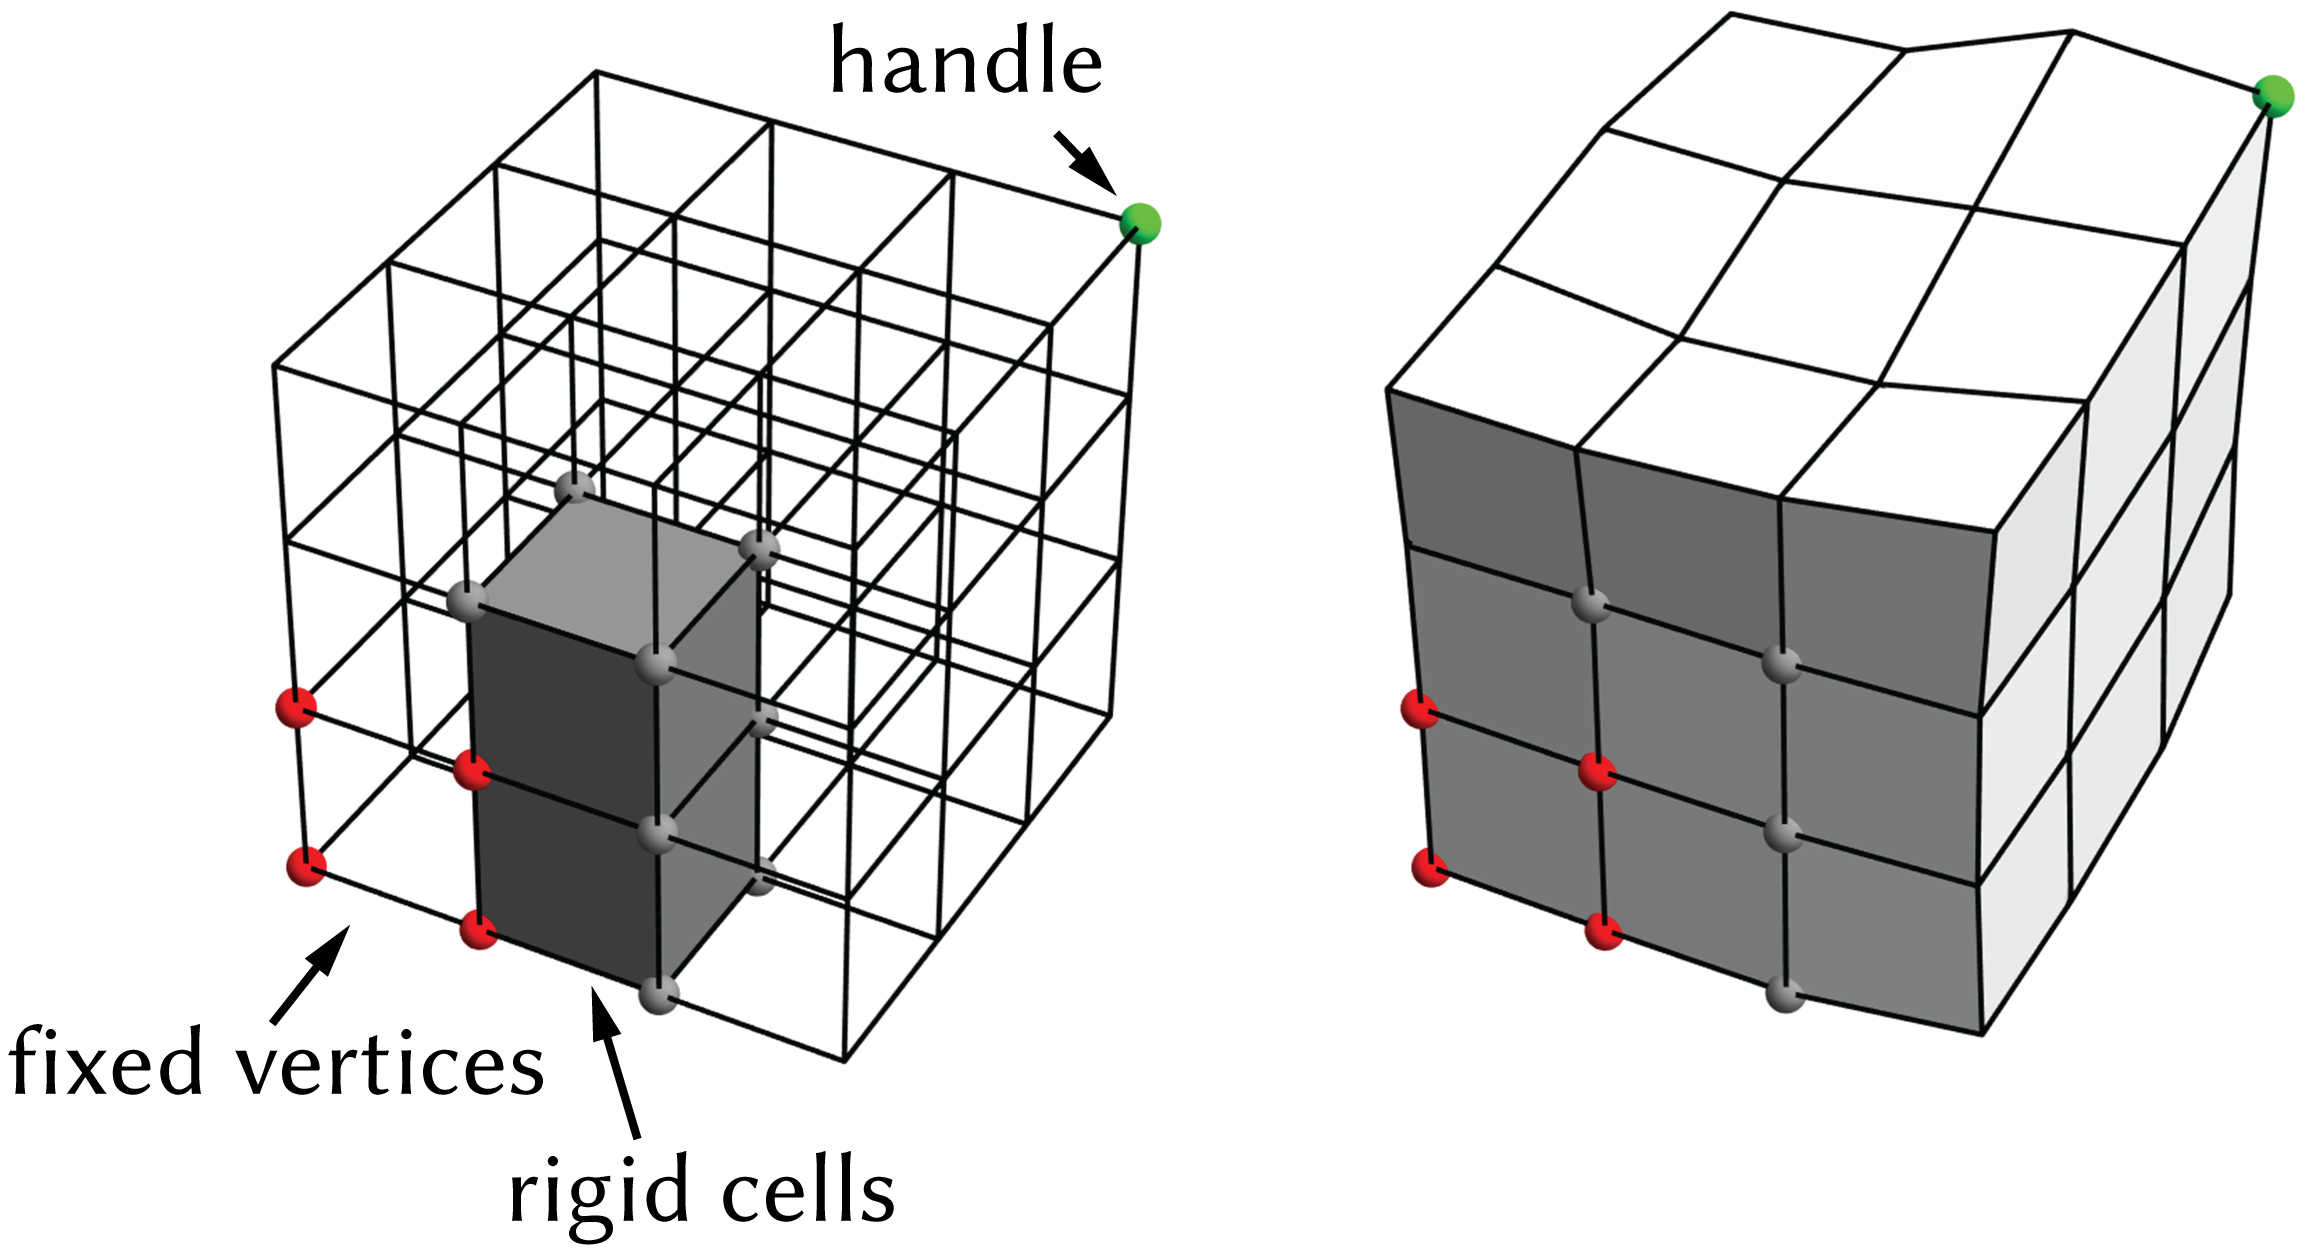
\includegraphics[width=0.65\textwidth]{chapters/understanding-metamaterial-mechanisms-FIG/19-3D-grid.png}
    \caption[Short figure name.]{Preview of a 3D deformed mechanism with 2 rigid cells.
    \label{fig:19-3D-grid}}
\end{figure}


\subsection{Practical extensions}

There are several practical extensions to our work, that concern the editor, including the simulation and generation of mechanisms. 

\subsubsection{Adapt to material properties}
We used an idealized simulation that does not incorporate engineering factors such as material properties or friction. We did so to focus on the interaction between geometric constraints within a mechanism, which could be missed when taking mechanical factors such as transmission loss into account. While the mechanical properties can be optimized (e.g., through high-resolution 3D printing), the underlying constraints are inherent to the geometry. Material properties could be used to expand the repertoire of transformations. Including other types of simulation such as finite element analysis would be one beneficial extension of the editor. This would also allow us to adaptively change the stiffness, thus actuation force, of a mechanism. This can be achieved by merging cells.

\subsubsection{Multiple layers with the same input}
Many practical applications such as a multi-legged Jansen walker or a robotic gripper require that multiple layers of mechanisms move in concert with each other, i.e., they use same coinciding input.  While our current editor only supports a creating a single layer at a time, they could be merged using any CAD tool.

\subsubsection{Extending to different cell types}
Our constraint graph, and consequently our optimization algorithm, hold true for other cell suggested previously in Section~\ref{section:shear-cell}, such as rotated and pre-sheared cells. Our editor only needs to be extended slightly to edit such cells.
 
\begin{figure} [h]
    \centering
    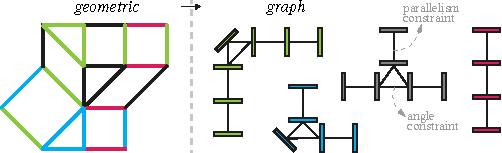
\includegraphics[width=0.9\textwidth]{chapters/understanding-metamaterial-mechanisms-FIG/20-generalized-2D-constraint-graph.pdf}
    \caption[Short figure name.]{Our constraint graph generalizes to the cells we introduces in Section~\ref{section:shear-cell}.
    \label{fig:20-generalized-2D-constraint-graph}}
\end{figure}

\subsubsection{Considering temporal changes}
We were concerned with the spatial transformation of metamaterial mechanisms. An extension of the optimization would be to also include a temporal component. Considering the speed of transformation would allow features such as keyframing and easing of motion. We plan to investigate this interesting aspect by adapting our error function and add keyframing to the editor.


\section{Conclusions}

We analyzed metamaterial mechanisms with respect to their topological constraints. Although the basic cells in this work (shear and rigid cells) are simple, connecting them creates complex interactions. We investigated these interactions, which we modeled as a constraint graph. This abstract graph representation allows us to explore metamaterials on a more abstract level and avoid having to rely on the raw cell structure which exhibits a prohibitively large search space. Consequently, we implemented our knowledge as a computational design tool for the automatic generation of such mechanisms. 

On a higher level, we think of our work as the first step towards what we like to call \textit{heterogenous mechanical metamaterials}. We define them as metamaterials that consist of \textit{different types} of cells. Most often metamaterials consist of cells that are topologically equivalent; all cells have the same function, but they can vary in parameter. Metamaterial mechanisms is one example of a material that consists of \textit{topologically different cells}. They exhibit interesting behavior yet the interactions between cells are hard to understand. In the future, we will go step-wise towards investigating more of these heterogenous metamaterials by creating generic tools that allow researchers to investigate combinations of different types of cells from related work. 


\pagebreak

\section{Appendix A: Enumerating all unique mechanisms}
\label{appendix:unique-mechanisms}

As noted in Section~\ref{section:search-space}, all edges in a row or column necessarily belong to a single connected component. Starting with an empty $n \times m$ grid we have $n+m$ connected components. Introducing a rigid cell joins two connected components and removes one degree of freedom. Suppose we want to enumerate all unique mechanisms with $k$ degrees of freedom. This amounts to $k$ connected components where we differentiate between $x$ empty columns, $y$ empty rows and $z$ components formed by merging rows and columns using rigid cells. There are $\binom{n}{x}$ ways to choose the columns and $\binom{m}{y}$ ways to choose the rows. The remaining $m-y$ rows and $n-x$ columns can be arbitrarily partitioned into $z$ sets. The Stirling number of the second kind counts the number of these partitions as $S(n-x,\ z)$ and $S(m-y,z)$ where we use the convention $S\left(a,b\right)=0$ for $a<b$. The $z$ sets of rows and columns can be connected in $z!$ ways. This gives 
$$G^{n,m}\left(x,y,z\right)=\ \binom{n}{x}\ \binom{m}{y}S\left(n-x,\ z\right)\ S\left(m-y,z\right)\ z!$$
different possibilities. Summing over all values for $x,\ y$ and $z$ we obtain the number of all possible unique mechanisms on a $n \times m$ grid. We empirically verified this number by analyzing all possible configurations on grids with $n<5$.

\pagebreak

% \appendix

\section{Appendix B: Example transformations}
\label{appendix:example-transformations}
\begin{figure} [h!]
    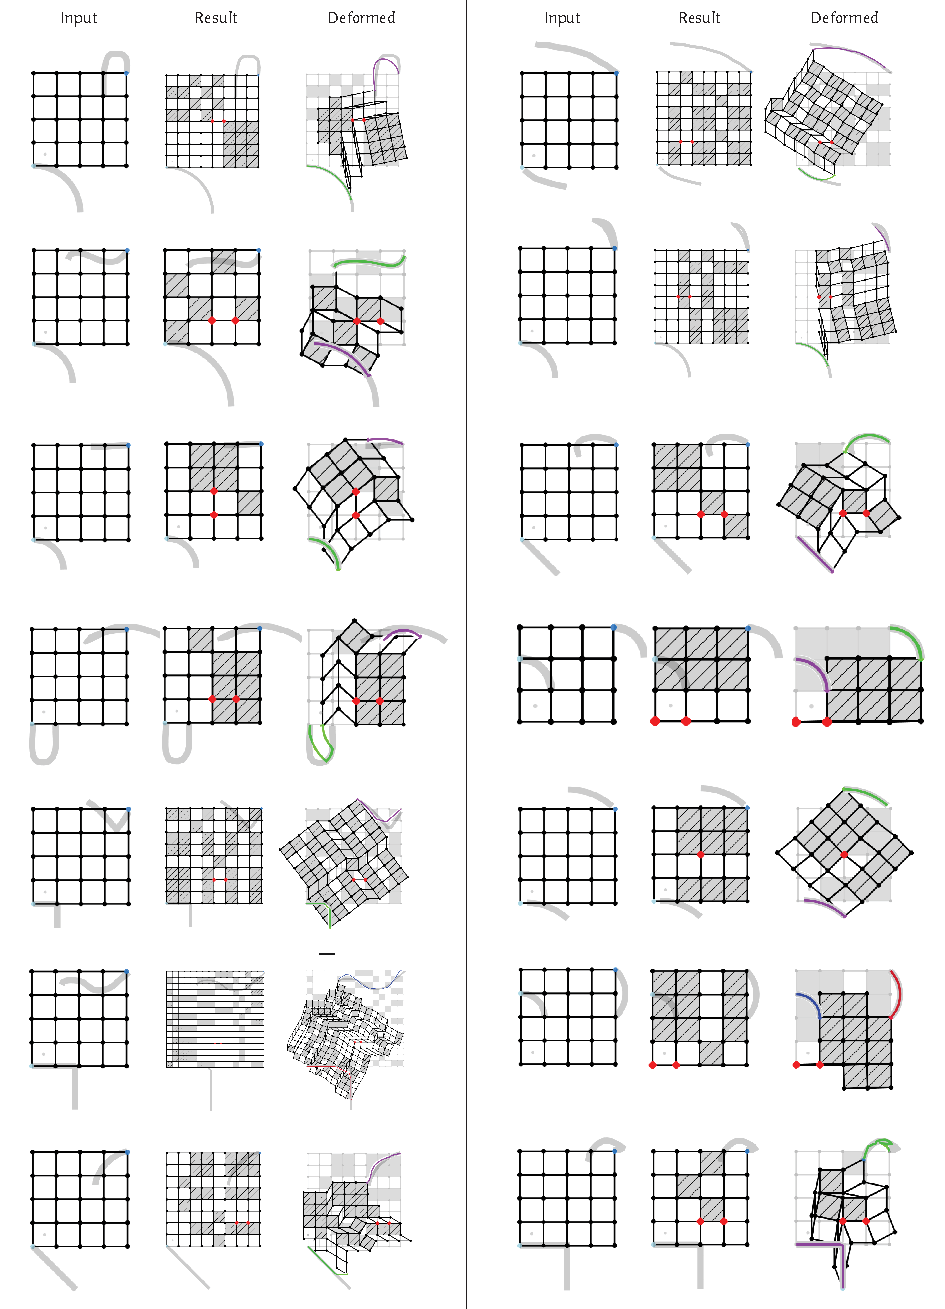
\includegraphics[width=\textwidth]{chapters/understanding-metamaterial-mechanisms-FIG/21-optimization-results.pdf}
    \caption[Short figure name.]{Examples of auto-generated metamaterial mechanisms.
    \label{fig:21-optimization-results}}
\end{figure}


% \begin{figure} [h]
%     \includegraphics[width=\textwidth]{chapters/understanding-metamaterial-mechanisms-FIG/}
%     \caption[Short figure name.]{
%     \label{fig:}}
% \end{figure}